%\newenvironment{limitscope}{}{}
\begin{limitscope}
\tikzset
{
    treenode/.style = {circle, draw=black, align=center, minimum size=1cm},
    subtree/.style  = {isosceles triangle, draw=black, align=center, minimum height=0.5cm, minimum width=1cm, shape border rotate=90, anchor=north},
    subtree1/.style  = {isosceles triangle, draw=black, align=center, minimum height=0.5cm, minimum width=0.5cm, shape border rotate=90, anchor=north},
    process/.style={rectangle, minimum width=2cm, minimum height=1cm, align=center, text width=2cm, draw},
    connector/.style={circle, minimum size=1cm, align=center, text width=0.5cm, draw},
    arrow/.style={thick, ->, >=stealth}
}
%%%%% icdcn macros - begin
\newcommand{\terminalnode}{terminal node}
\newcommand{\targetnode}{target node}
\newcommand{\accesspath}{access-path}
\newcommand{\nullFlag}{null-flag}
\newcommand{\intentFlag}{intent-flag}
\newcommand{\deleteFlag}{delete-flag}
\newcommand{\promoteFlag}{promote-flag}
\newcommand{\anchornode}{anchor node}
\newcommand{\injection}{injection}
\newcommand{\discovery}{discovery}
\newcommand{\cleanup}{cleanup}

\newcommand{\Search}{\textsc{Search}}
\newcommand{\Insert}{\textsc{Insert}}
\newcommand{\Delete}{\textsc{Delete}}
\newcommand{\Seek}{\textsc{Seek}}
\newcommand{\FindSmallest}{\textsc{FindSmallest}}
\newcommand{\Inject}{\textsc{Inject}}
\newcommand{\FindAndMarkSuccessor}{\textsc{FindAndMarkSuccessor}}
\newcommand{\RemoveSuccessor}{\textsc{RemoveSuccessor}}
\newcommand{\Cleanup}{\textsc{Cleanup}}
\newcommand{\InitializeTypeAndUpdateMode}{\textsc{InitializeTypeAndUpdateMode}}
\newcommand{\UpdateMode}{\textsc{UpdateMode}}
\newcommand{\HelpTargetNode}{\textsc{HelpTargetNode}}
\newcommand{\HelpSuccessorNode}{\textsc{HelpSuccessorNode}}
\newcommand{\MarkChildEdge}{\textsc{MarkChildEdge}}
\newcommand{\remove}[1]{}


\newcommand{\snodeone}{\mathbb{R}}
\newcommand{\snodetwo}{\mathbb{S}}
\newcommand{\snodethree}{\mathbb{T}}
\newcommand{\skey}[1]{\infty_{#1}}


\newcommand{\myleft}{le\!f\!t}
\newcommand{\myright}{right}
\newcommand{\myparent}{parent}

%%%%% icdcn macros - end
\section{The Lock-Free Algorithm}
\label{sec:icdcn-algorithm}

For ease of exposition, we describe our algorithm assuming no memory reclamation.

\subsection{Overview of the Algorithm}

Every operation in our algorithm uses \emph{seek} function as a subroutine. The seek function traverses the  tree from the root node until it either finds the target key or reaches a non-binary node whose next edge to be followed points to a null node. We refer to the path traversed by the operation during the seek  as the \emph{\accesspath}, and the last node in the \accesspath{} as the \emph{\terminalnode}. The operation then compares the target key with the stored key (the key present in the \terminalnode). Depending on the result of the comparison and the type of the operation, the operation either terminates or moves to the execution phase. In certain cases in which a key may have moved upward along the \accesspath, the seek function may have to restart and traverse the tree again; details about restarting are provided later. We now describe the next steps for each of the operations one-by-one.

\paragraph*{Search} 
A search operation starts by invoking seek operation. It returns \true{} if the stored key matches the target key and \false{} otherwise. 

\paragraph*{Insert}
\begin{figure}[htp]
\centering
{
	\begin{tikzpicture}
		\newcommand\XA{0}
		\newcommand\YA{0}
		\node (x)		[treenode,fill=black!20] 									at (\XA,\YA)       							{$U$ \\ 50};
		\node (S1)	[subtree] 																at ([shift=({-1.5,-0.75})]x)  	{\Large $\alpha$};
		\node (gnd)	[ground] 																	at ([shift=({1.5,-0.75})]x)			{}; 
		\node (l1) [rectangle,align=center,minimum size=1cm] 	at (\XA-1.5,\YA) 								{\large terminal \\ \large node};
		\node (l2) [rectangle,align=center,minimum size=1cm] 	at (\XA+2,\YA-2.0) 					{\large injection \\ \large point};
		\path[every node/.style={font=\sffamily\small}]
		(\XA,\YA+1) edge[->] 																	node 														{} (x)
		(x) 				edge[->]																	node 														{} (S1.north)
		(x) 				edge[->,thick]														node 														{} (gnd);

		\path[every node/.style={font=\sffamily\small}]
		(\XA+2.0,\YA) edge[->,semithick, double] node [above, outer sep=3pt] {\large \texttt insert 55} (\XA+4.5,\YA);
		\renewcommand\XA{6.5}
		\renewcommand\YA{0}
		\node (x1)		[treenode,fill=black!20] 								at (\XA,\YA)       							{$U$ \\ 50};
		\node (S2)	[subtree] 																at ([shift=({-1.5,-.75})]x1)  	{\Large $\alpha$};
		\node (y)		[treenode,fill=black!20] 									at ([shift=({2,-1.25})]x1)   		{$V$ \\ 55};
		\node (l2) [rectangle,align=center,minimum size=1cm] 	at (\XA+3.5,\YA-1.25) 					{\large new \\ \large node};
    \node (gnd1)	[ground] 																at ([shift=({1.5,-0.75})]y)			{}; 
		\node (gnd2)	[ground] 																at ([shift=({-1.5,-0.75})]y)		{}; 
		
		\path[every node/.style={font=\sffamily\small}]
		(\XA,\YA+1) edge[->] 																	node 														{} (x1)
		(x1) 				edge[->]																	node 														{} (S2.north)
		(x1) 				edge[->,thick]														node 														{} (y)
		(y)         edge[->,thick]                						node          									{} (gnd1)
		(y)         edge[->,thick]                						node          									{} (gnd2);
	\end{tikzpicture}
}
\caption{An illustration of an insert operation.}
\label{fig:icdcn-insert}
\end{figure}
An insert operation ((shown in \figref{icdcn-insert})) starts by invoking seek operation. It returns \false{} if the target key matches the stored key; otherwise, it moves to the execution phase. In the execution phase, it attempts to insert the key into the tree as a child node of the last node in the \accesspath{} using a \CAS{} instruction. If the instruction succeeds, then the operation returns \true{}; otherwise, it restarts by invoking the seek function again.

\paragraph*{Delete} 
\begin{figure}[htp]
\centering
{
	\begin{tikzpicture}[scale=0.6, transform shape,mylabel/.style={thin, draw=black, align=center, minimum width=0.3cm, minimum height=0.3cm,fill=white}]
		\newcommand\XA{-3}
		\newcommand\YA{0}
		\node (x)		[treenode] 																at (\XA,\YA)       					{$V$ \\ 100};
		\node (y)		[treenode, fill=black!20] 								at (\XA-1.5,\YA-1.5) 				{$U$ \\ 50};
		\node (a)		[subtree] 																at (\XA+2,\YA-1)      			{\Large $\alpha$};
		\node (b)		[subtree] 																at (\XA-3,\YA-2.5)    			{\Large $\beta$};
		\node (gnd)	[ground] 																	at (\XA+0.5,\YA-2.5)				{}; 
		\node (xl) 	[rectangle,align=center,minimum size=1cm] at (\XA-2,\YA) 							{\large \targetnode's \\ \large parent};
		\node (yl) 	[] 																				at (\XA-3.25,\YA-1.5) 			{\large \targetnode};
		\draw[->] (x) -- node[mylabel] {$\boldsymbol{i}$} (y);
		\draw[->] (y) -- node[mylabel] {$\boldsymbol{d}$} (b.north);
		\draw[->] (y) -- node[mylabel] {$\boldsymbol{d}$} (gnd);
		\path[every node/.style={font=\sffamily\small}]
		(\XA,\YA+1) edge[->] 																	node 												{} (x)
		%(x) 				edge[->] 																	node[below]  								{\Large $\boldsymbol{i}$} (y)
		(x) 				edge[->] 																	node 				 								{} (a.north);
		%(y) 				edge[->]																	node[below]  								{\Large $\boldsymbol{d}$} (b.north)
		%(y) 				edge[->]																	node[below]  								{\Large $\boldsymbol{d}$} (gnd);

		\path[every node/.style={font=\sffamily\small}]
		(\XA+1.5,\YA) edge[->,semithick, double] 							node [above, outer sep=3pt] {\large \texttt delete 50} (\XA+4,\YA);
		\node (ix)	[treenode] 																at (\XA+6,\YA) 							{$V$ \\ 100};
		\node (ib)	[subtree] 																at (\XA+4.5,\YA-1)					{\Large $\beta$};
		\node (ia)	[subtree] 																at (\XA+7.5,\YA-1) 					{\Large $\alpha$};

		\path[every node/.style={font=\sffamily\small}]
		(\XA+6,\YA+1) 	edge[->] 															node 												{} (ix)
		(ix) 				edge[->] 																	node 												{} (ib.north)
		(ix) 				edge[->] 																	node 												{} (ia.north);

		%% legend
		\node (l1) 																						at (\XA+4.5,\YA-3){\Large $\boldsymbol{i}$  - \Large intent flag set};
		\node (l2) 																						at (\XA+4.5,\YA-3.5){\Large $\boldsymbol{d}$  - \Large delete flag set};
		\node [thin, draw=black, align=center, minimum width=5cm, minimum height=1.25cm] at (\XA+5,\YA-3.15) {};	
	\end{tikzpicture}
}
\caption{An illustration of a simple delete operation.}
\label{fig:simple}
\end{figure}
\begin{figure}[htp]
\centering
{
	\begin{tikzpicture}[scale=0.55, transform shape,mylabel/.style={thin, draw=black, align=center, minimum width=0.3cm, minimum height=0.3cm,fill=white}]
		\newcommand\XA{0}
		\newcommand\YA{0}
		\node (x)		[treenode, fill=black!20] 	at (-6,0)       							{$U$ \\ 50};
		\node (a)		[subtree] 									at (-7.5,-1)  								{\Large $\alpha$};
		\node (y0)	[treenode] 									at (-4,-1.5) 									{$V$ \\ 100};
		\node (y1)	[treenode]									at (-5.5,-3)									{$W$ \\ 60}; 
		\node (b)		[subtree] 									at (-3,-2.5)    							{\Large $\beta$};
		\node (y2)	[treenode]									at (-7,-4.5)									{$X$ \\ 55}; 
		\node (g)		[subtree] 									at (-4,-4)   									{\Large $\gamma$};
		\node (gnd)	[ground] 										at (-8.5,-5.75)									{}; 
		\node (o)		[subtree] 									at (-5.5,-5.5)  							{\Large $\omega$};
		\node (x1) 	[] 													at (-7.75,0) 									{\large \targetnode};
		\node (y1l) [rectangle,align=center,minimum size=1cm] at (-7.5,-3) 		{\large successor node's \\ \large parent};
		\node (y2l) [rectangle,align=center,minimum size=1cm] at(-8.5,-4.5) 	{\large successor \\ \large node};
		%\node (i)																at (-5.8,1.1)							{\Large $\boldsymbol{i}$};
		%\node (p)																at (-7.75,-5.4)								{\Large $\boldsymbol{p}$};
		
		\draw[->] (-6, 1.5) -- node[mylabel] {$\boldsymbol{i}$} (x);
		\draw[->] (x) -- node[mylabel] {$\boldsymbol{d}$} (y0);
		\draw[->] (x) -- node[mylabel] {$\boldsymbol{d}$} (a.north);
		\draw[->] (y2) -- node[mylabel] {$\boldsymbol{p}$} (gnd);
		\draw[->] (y2) -- node[mylabel] {$\boldsymbol{p}$} (o.north);
		
		
		\path[every node/.style={font=\sffamily\large}]
		%(-6, 1.5) edge[->] 											node 													{} (x)
		%(x) 		edge[->] 												node[below] 									{\Large $\boldsymbol{d}$} (y0)
		%(x) 		edge[->]												node[below] 									{\Large $\boldsymbol{d}$} (a.north)
		(y0) 		edge[->] 												node 													{} (y1)
		(y0) 		edge[->] 												node 													{} (b.north)
		(y1) 		edge[->] 												node 													{} (y2)
		(y1) 		edge[->] 												node 													{} (g.north);
		%(y2) 		edge[->]												node[below] 									{} (gnd)
		%(y2) 		edge[->]												node[below] 									{\Large $\boldsymbol{p}$} (o.north);

		\path[every node/.style={font=\sffamily\small}]
		(-3.25, 0) edge[->,semithick, double] node [above, outer sep=3pt] 		{\large \texttt delete 50} (-0.75, 0);

		\node (ix)	[treenode] 									at (1,0)       								{$U\prime$ \\ 55};
		\node (ia)	[subtree] 									at (-0.5,-1)  								{\Large $\alpha$};
		\node (iy0)	[treenode] 									at (3,-1.5) 									{$V$ \\ 100};
		\node (iy1)	[treenode]									at (1.5,-3)										{$W$ \\ 60}; 
		\node (ib)	[subtree] 									at (4,-2.5)    								{\Large $\beta$};
		\node (io)	[subtree]										at (0,-4)											{\Large $\omega$}; 
		\node (ignd)[subtree] 									at (3,-4)   									{\Large $\gamma$};

		\path[every node/.style={font=\sffamily\small}]
		(1, 1.5) 	edge[->] 											node 													{} (ix)
		(ix) 		edge[->] 												node 													{} (iy0)
		(ix) 		edge[->] 												node 													{} (ia.north)
		(iy0) 	edge[->] 												node 													{} (iy1)
		(iy0) 	edge[->] 												node 													{} (ib.north)
		(iy1) 	edge[->] 												node 													{} (io.north)
		(iy1) 	edge[->] 												node 													{} (ignd.north);

		%% legend
		\node (l1) 															at (-1.5, -5.8)								{\Large $\boldsymbol{i}$  - \Large intent flag set};
		\node (l2) 															at (2.5, -5.8)								{\Large $\boldsymbol{d}$  - \Large delete flag set};
		\node (l3) 															at (-1.25, -6.3)							{\Large $\boldsymbol{p}$  - \Large promote flag set};
		\node [thin, draw=black, align=center, minimum width=8.1cm, minimum height=1.25cm] at (0.5, -6.1) {};
	\end{tikzpicture}
}
\caption{An illustration of a complex delete operation.}
\label{fig:complex}
\end{figure}
A delete operation starts by invoking seek function. It returns \false{} if the stored key does not match the target key; otherwise, it moves to the execution phase. In the execution phase, it attempts to remove the key stored in the \terminalnode{} of the \accesspath. There are two cases depending on whether the \terminalnode{} is a binary node (has two children) or not (has at most one child). In the first case, the operation is referred to as \emph{complex delete operation}. In the second case, it is referred to as \emph{simple delete operation}. In the case of simple delete (shown in \figref{icdcn-simple}), the \terminalnode{} is removed by changing the pointer at the parent node of the \terminalnode. In the case of complex delete (shown in \figref{icdcn-complex}), the key to be deleted is replaced with the \emph{next largest} key in the tree, which will be stored in the \emph{leftmost node} of the \emph{right subtree} of the \terminalnode.

\subsection{Details of the Algorithm}

\begin{figure}[htp]
\centering
{
	\begin{tikzpicture}[scale=0.625, transform shape]
	\newcommand\XA{0}
	\newcommand\YA{0}
	\newcommand\XB{\XA-1}
	\newcommand\YB{\YA-3.8}
	\node (R)			[treenode] 									at (\XA,\YA)       						{$\snodeone$ \\ $\infty$$_0$};
	\node (gnd)		[ground] 										at ([shift=({-1.5,-1})]R)				{};  
	\node (S)			[treenode] 									at ([shift=({1.5,-1.35})]R)			{$\snodetwo$ \\ $\infty$$_1$};
	\node (gndls)	[ground] 										at ([shift=({-1.5,-1})]S)				{}; 
	\node (T)			[treenode] 									at ([shift=({1.5,-1.35})]S)			{$\snodethree$ \\ $\infty$$_2$};
%	\node (gndlt)	[ground] 										at ([shift=({-1,-1})]T)				{};  
	\node (gndt)	[ground] 										at ([shift=({1.5,-1})]T)				{};  


	\path[every node/.style={font=\sffamily\small}]
	(R) 					edge[->] 										node  												{} (S)
	(R) 					edge[->] 										node 				 									{} (gnd)
	(S)						edge[->] 										node 													{} (gndls)
	(S)						edge[->] 										node 													{} (T)
%	(T)						edge[->] 										node 													{} (gndlt)
	(T)						edge[->] 										node 													{} (gndt);
	\renewcommand\XA{0}
	\renewcommand\YA{-4}
	\renewcommand\XB{\XA+2}
	\renewcommand\YB{\YA-6.8}
	\node (x)		[treenode] 									at (\XA,\YA)       						{$U$ \\ 10};
	\node (S1)	[subtree1] 									at ([shift=({-1.5,-0.5})]x)  		{\Large $\alpha$};
	\node (y0)	[treenode] 									at ([shift=({3,-0.5})]x) 			{$V$ \\ 100};
	\node (y1)	[treenode,fill=black!20]		at ([shift=({-1.5,-1})]y0)		{$W$ \\ 60}; 
	\node (S2)	[subtree1] 									at ([shift=({2,-0.5})]y0)   	{$\beta$};
	\node (S3)	[subtree1] 									at ([shift=({-1.5,-1})]y1)  		{\Large $\gamma$};
	\node (y2)	[treenode]									at ([shift=({1.5,-1})]y1)			{$X$ \\ 55}; 
	\node (y3)	[treenode]									at ([shift=({-1,-1.5})]y2)		{$Y$ \\ 50}; 
	\node (S4)	[subtree1] 									at ([shift=({1.5,-0.5})]y2)  	{\Large $\omega$};
	\node (y4)	[treenode,fill=black!20]		at ([shift=({-1,-1.5})]y3)		{$Z$ \\ 40};
	\node (S5)	[subtree1] 									at ([shift=({1.5,-0.5})]y3)  	{\Large $\delta$}; 
	\node (gnd)	[ground] 										at ([shift=({-1,-1})]y4)			{}; 
	\node (S6)	[subtree1] 									at ([shift=({1.5,-0.5})]y4)  	{\Large $\sigma$}; 
	\node (y1l) [rectangle,align=center,minimum size=1cm] at (\XA+0.25,\YA-1.4) 				{\large anchor \\ \large node};
	\node (y4l) [] 													at (\XA-1.0,\YA-5.4) 				{\large \terminalnode};
	\node (x1) 	[rectangle,align=center,minimum size=1cm]at (\XA-1.75,\YA-6.75) 	{\large injection point};

	\path[every node/.style={font=\sffamily\large}]
	%(\XA,\YA+1) 	edge[->,thick] 						node 													{} (x)
	(T)			edge[->,dotted] 								node 													{} (x)
	(x) 		edge[->]												node 													{} (y0)
	(x) 		edge[->]												node 													{} (S1.north)
	(y0) 		edge[->]												node 													{} (y1)
	(y0) 		edge[->]												node 													{} (S2.north)
	(y1) 		edge[->]												node 													{} (S3.north)
	(y1) 		edge[->]												node 													{} (y2)
	(y2) 		edge[->]												node 													{} (y3)
	(y2) 		edge[->]												node 													{} (S4.north)
	(y3) 		edge[->]												node 													{} (y4)
	(y3) 		edge[->]												node 													{} (S5.north)
	(y4) 		edge[->]												node 				 									{} (gnd)
	(y4) 		edge[->]												node 													{} (S6.north);
		
 \end{tikzpicture}
}
\caption{Nodes in the access path of seek along with sentinel keys and nodes ($\infty_0 < \infty_1 < \infty_2$)}
\label{fig:sentinelAndSeek}
\end{figure}



As in most algorithms, we use sentinel keys and three sentinel nodes to handle the boundary cases easily.  The structure of an empty tree with only sentinel keys (denoted by $\skey{0}$, $\skey{1}$ and $\skey{2}$ with $\skey{0} < \skey{1} < \skey{2}$) and sentinel nodes (denoted by $\snodeone$, $\snodetwo$ and $\snodethree$) is shown in \figref{icdcn-sentinelAndSeek}.


Our algorithm, like the one in~\cite{NatMit:2014:PPoPP}, operates at edge level. A delete operation obtains ownership of the edges it needs to work on by marking them. To enable marking, we steal bits from the child addresses of a node. Specifically, we steal \emph{three} bits from each child address to distinguish between three types of marking: 
%%
\begin{enumerate*}[label=(\roman*)]
\item marking for \emph{intent}, 
\item marking for \emph{deletion} and 
\item marking for \emph{promotion}.
\end{enumerate*}
%%
The three bits are referred to as \emph{\intentFlag}, \emph{\deleteFlag} and \emph{\promoteFlag}. To avoid the ABA problem, as in Howley and Jones~\cite{HowJon:2012:SPAA}, we use \emph{unique} null pointers. To that end, we steal another bit from the child address, referred to as \emph{\nullFlag}, and use it to indicate whether the address field contains a null or a non-null value. So, when an address changes from a non-null value to a null value, we only set the \nullFlag{} and the contents of the address field are not otherwise modified. This ensures that all null pointers are unique.

Finally, we also steal a bit from the key field to indicate whether the key stored in a node is the original key or the replacement key. This information is used in a complex delete operation to coordinate helping among processes.


We next describe the details of the seek function, which is used by all operations (search as well as modify) to traverse the tree after which we describe the details of 
the execution phase of insert and delete operations.

\subsubsection{The Seek Phase}
A seek function keeps track of the node in the \accesspath{} at which it took the last ``right turn'' (\emph{i.e.}, it last followed a right edge). Let this ``right turn'' node be referred to as \emph{\anchornode} when the traversal reaches the \terminalnode{}. Note that the \terminalnode{} is the node whose key matched the target key or whose next child edge is set to a null address. For an illustration, please see \figref{icdcn-sentinelAndSeek}. In the latter case (stored key does not match the target key), it is possible that the key may have moved up in the tree. To ascertain that the seek function did not miss the key because it may have moved up during the traversal, we use the following set of conditions that are \emph{sufficient} (but not necessary) to guarantee that the seek function did not miss the key. First, the \anchornode{} is still part of the tree. Second, the key stored in the \anchornode{} has not changed since it first encountered the \anchornode{} during the (current) traversal. To check for the above two conditions, we determine whether the \anchornode{} is undergoing removal (either delete or promote flag set) by examining its right child edge. We discuss the two cases one-by-one.

\begin{enumerate}[leftmargin=*, label=(\alph*), noitemsep]

\item \emph{Right child edge not marked:}
In this case, the \anchornode{} is still part of the tree. We next check whether the key stored in the \anchornode{} has changed. If the key has not changed, then the seek function returns the results of the (current) traversal, which consists of three addresses:
\begin{enumerate*}[label=(\roman*)]
\item the address of the \terminalnode{}, 
\item the address of its parent, and
\item the null address stored in the child field of the \terminalnode{} that caused the traversal to terminate.
\end{enumerate*}
The last address is required to ensure that an insert operation works correctly (specifically to ascertain that the child field of the \terminalnode{} has not undergone any change since the completion of the traversal). We refer to it as the \emph{injection point} of the insert operation. On the other hand, if the key has changed, then the seek function restarts from the root of the tree. 


\item \emph{Right child edge marked:}
In this case, we compare the information gathered in the current traversal about the \anchornode{} with that in the previous traversal, if one exists. Specifically, if the \anchornode{} of the previous traversal is same as that of the current traversal  and the keys found in the \anchornode{} in the two traversals also match, then the seek function terminates, but returns the results of the previous traversal (instead of that of the current traversal). This is because the \anchornode{} was definitely part of the tree during the previous traversal since it was reachable from the root of the tree at the beginning of the current traversal. Otherwise, the seek function restarts from the root of the tree.  
\end{enumerate}

The seek function also keeps track of the \emph{second-to-last} edge in the \accesspath{} (whose endpoints are the parent and grandparent nodes of the \terminalnode), which 
is used for helping, if there is a conflict. For insert and delete operations, we refer to the \terminalnode{} as the \emph{\targetnode}. 

\subsubsection{The Execution Phase of an Insert Operation}

\begin{figure}[htp]
\centering
{
	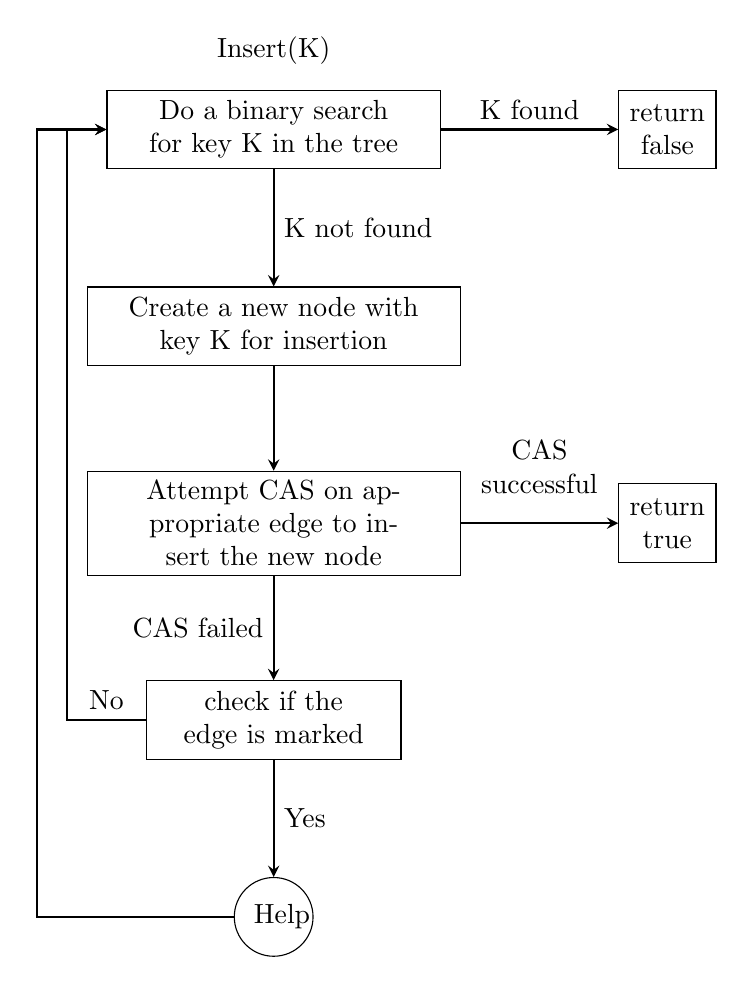
\begin{tikzpicture}
	\node (p0) [] {Insert(K)};
	\node (p1) [process, below of=p0, text width=4cm] {Do a binary search for key K in the tree};
	\node (p2) [process, below of=p1, yshift=-1.5cm, text width=4.5cm] {Create a new node with key K for insertion};
	\node (p3) [process, below of=p2, yshift=-1.5cm, text width=4.5cm] {Attempt CAS on appropriate edge to insert the new node};
	\node (retF) [process, right of=p1, xshift=4cm, text width=1cm, minimum width=1cm] {return false};
	\node (p4) [process, below of=p3, yshift=-1.5cm, text width=3cm] {check if the edge is marked};
	\node (retT) [process, right of=p3, xshift=4cm, text width=1cm, minimum width=1cm] {return true};
	\node (h1) [connector, below of=p4, yshift=-1.5cm] {Help};



	\draw [arrow] (p1) -- node[anchor=west] {K not found} (p2);
	\draw [arrow] (p1) -- node[anchor=south] {K found} (retF);
	\draw [arrow] (p2) -- node {} (p3);
	\draw [arrow] (p3) -- node[anchor=east] {CAS failed} (p4);
	\draw [arrow] (p3) -- node[anchor=south, align=center, yshift=0.25cm] {CAS \\ successful} (retT);
	\draw [arrow] (p4) -- node[anchor=west] {Yes} (h1);
	\draw [arrow] (p4.west) -- ++(-1,0)  node[anchor=south,pos=0.5] {No} |- (p1.west);
	\draw [arrow] (h1.west) -- ++(-2.5,0) |- node[anchor=south] {} (p1.west);
	\end{tikzpicture}
}
\caption{\ICDCN{} - Sequence of steps in an insert operation \label{fig:icdcn-flowInsert}}
\end{figure}
In the execution phase, an insert operation creates a new node containing the target key. It then adds the new node to the tree at the injection point using a \CAS{} instruction. If the \CAS{} instruction succeeds, then (the new node becomes a part of the tree and) the operation terminates; otherwise, the operation determines if it failed because of a \emph{conflicting} delete operation in progress. If there is no conflicting delete operation in progress, then the operation restarts from the seek phase; otherwise it performs helping and then restarts from the seek phase. \figref{icdcn-flowInsert} shows a  flow chart describing the sequence of steps of an insert operation.

\subsubsection{The Execution Phase of a Delete Operation}
The execution of a delete operation starts in \emph{\injection{} mode}. Once the operation has been injected into the tree, it advances to either \emph{\discovery{} mode} or \emph{\cleanup{} mode} depending on the type of the delete operation.


\paragraph*{Injection Mode}

In the \injection{} mode, the delete operation marks the three edges involving the \targetnode{} as follows:
%%
\begin{enumerate*}[label=(\roman*)]
\item It first sets the \intentFlag{} on the edge from the parent of the \targetnode{} to the \targetnode{} using a \CAS{} instruction.
\item It then sets the \deleteFlag{} on the left edge of the \targetnode{} using a \CAS{} instruction.
\item Finally, it sets the \deleteFlag{} on the right edge of the \targetnode{} using a \CAS{} instruction.
\end{enumerate*}
%%
If the \CAS{} instruction fails at any step, the delete operation performs helping, and either repeats the same step or restarts from the seek phase. Specifically, the delete operation repeats the same step when setting the \deleteFlag{} as long as the \targetnode{} has not been claimed as the successor node by another delete operation. In all other cases, it restarts from the seek phase.


We maintain the invariant that an edge, once marked, cannot be unmarked. After marking both the edges of the \targetnode{}, the operation checks whether the \targetnode{} is a binary node or not. If it is a binary node, then the delete operation is classified as complex; otherwise it is classified as simple. Note that the type of the delete operation cannot change once all the three edges have been marked as described above. If the delete operation is complex, then it advances to the \discovery{} mode after which it will advance to the \cleanup{} mode. On the other hand, if it is simple, then it directly advances to the \cleanup{} mode (and skips the \discovery{} mode). Eventually, the \targetnode{} is either removed from the tree (if simple delete) or replaced with a ``new'' node containing the next largest key (if complex delete). 

For a tree node $X$, let $X.\myparent$ denote its parent node, and $X.\myleft$ and $X.\myright$ denote its left and right child node, respectively. Also, hereafter in this section, let $T$ denote the \targetnode{} of the delete operation under consideration.

\paragraph*{Discovery Mode}
In the \discovery{} mode, a complex delete operation  performs the following steps:
%%
\begin{enumerate}[leftmargin=*, noitemsep]
%%
\item \textbf{Find Successor Key:} The operation locates the next largest key in the tree, which is the smallest key in the subtree rooted at the right child of $T$. We refer to this key as the \emph{successor key} and the node storing this key as the \emph{successor node}. Hereafter in this section, let $S$ denote the successor node. 
%%
\item \textbf{Mark Child Edges of Successor Node:} The operation sets the \promoteFlag{} on both the child edges of $S$ using a \CAS{} instruction. Note that the left child edge of $S$ will be null.  As part of marking the left child edge, we also store the address of $T$ (the \targetnode{}) in the edge. This is done to enable helping in case the successor node is obstructing the progress of another operation. 
%%
In case the \CAS{} instruction fails while marking the left child edge, the operation repeats from step~1 after performing helping if needed. On the other hand, if the \CAS{} instruction fails while marking the right child edge, then the marking step is repeated after performing helping if needed. 

%%
\item \textbf{Promote Successor Key:} The operation replaces the \targetnode's original key with the successor key. At the same time, it also sets the mark bit in the key to indicate that the current key stored in the \targetnode{} is the replacement key and not the original key.
%%
\item \textbf{Remove Successor Node:}  The operation removes $S$ (the successor node) by changing the child pointer at$S.\myparent$ that is pointing to $S$ to point to the right child of $S$ using a \CAS{} instruction. If the \CAS{} instruction succeeds, then the operation advances to the \cleanup{} mode. Otherwise, it performs helping if needed. It then finds $S$ again by performing another traversal of the tree starting from the right child of $T$. If the traversal fails to find $S$ (recall that the left edge of $S$ is marked for promotion and contains the address of $T$), then $S$ has already been removed from the tree by another operation as part of helping, and the delete operation advances to the \cleanup{} mode. On advancing to the \cleanup{} mode, the operation sets a flag in $T$  indicating that $S$ has been removed from the tree (and $T$ can now be replaced with a new node) so that other operations trying to help it know not to look for $S$.
\end{enumerate}

\figref{icdcn-flowDelete} shows a  flow chart describing the sequence of steps of a delete operation.
\begin{figure}[htp]
\centering
{
	\begin{tikzpicture}[scale=0.75, transform shape]
		\node (p0) 		{Delete(K)};
		\node (p1) 		[process, below of=p0, text width=6cm] {Do a binary search for key K in the tree};
		\node (p2) 		[process, below of=p1, yshift=-2cm, text width=6cm] {Mark left child edge for delete using CAS};
		\node (p3) 		[process, below of=p2, yshift=-2cm, text width=6cm] {Mark right child edge for delete using BTS. Check the children edges to determine simple or complex delete};
		\node (retF) 	[process, right of=p1, xshift=5.0cm, text width=1cm, minimum width=1cm] {return false};
		\node (p4) 		[process, below of=p3, yshift=-2cm, text width=6cm] {Attempt CAS to change the edge (parent, target node) to point to the non-null child};
		\node (retT) 	[process, right of=p4, xshift=5.0cm, text width=1cm, minimum width=1cm] {return true};
		%\node (C) 		[connector, right of=p3, xshift=5.5cm] {C};
		\node (h1) 		[connector, right of=p2, xshift=5.0cm] {Help};
		\node (h2) 		[connector, below of=p4, yshift=-2cm] {Help};



		\draw [arrow] (p1) -- node[anchor=west] {K found} (p2);
		\draw [arrow] (p1) -- node[anchor=south] {K not found} (retF);
		\draw [arrow] (p2) -- node[anchor=west, align=center] {CAS successful} (p3);
		\draw [arrow] (p2) -- node[anchor=south, align=center, yshift=0.25cm] {CAS \\ failed} (h1);
		\draw[-latex] (h1) to [out=90,in=330,looseness=1] (p1.east);
		\draw [arrow] (p3) -- node[anchor=east] {simple} (p4);
		%\draw [arrow] (p3) -- node[anchor=south] {Complex} (C);
		\draw [arrow] (p4) -- node[anchor=south, align=center, yshift=0.25cm] {CAS \\ successful} (retT);
		\draw [arrow] (p4) -- node[anchor=east] {CAS failed} (h2);
		%\draw [arrow] (h2.west) -- ++(-0,0) |- node[anchor=south] {} (p4.west);
		\draw[-latex] (h2.east) to [out=0,in=0,looseness=1.5] (p4.east);
	%\end{tikzpicture}

	%\begin{tikzpicture}[scale=0.7, transform shape]
	%\node (C) [connector,xshift=11cm] {C};
	%\node (p1) [process, below of=C, yshift=-2cm, text width=6cm] {Find Successor: smallest key in the right subtree};
	\node (p1c) [process, xshift=11cm,text width=6cm] {Find Successor: smallest key in the right subtree};
	\draw [arrow] (p3.east) -- ++(4,0) |- node[anchor=south] {Complex} (p1c.west);
	\node (p2) [process, below of=p1c, yshift=-2cm, text width=6cm] {Mark left child edge for promotion using CAS};
	\node (p3) [process, below of=p2, yshift=-2cm, text width=6cm] {Mark right child edge for promotion using BTS. Promote successor's key by copying it to the target node using a simple write};
	\node (h1) [connector, right of=p2, xshift=5cm] {Help};
	\node (p4) [process, below of=p3, yshift=-2cm, text width=6cm] {Attempt CAS to change the edge (successor parent,successor) to point to the right child of successor};
	\node (p5) [process, below of=p4, yshift=-2cm, text width=6cm] {Create a fresh copy of the target node with the new key and its children edges unmarked};
	\node (h2) [connector, right of=p4, xshift=5cm] {Help};
	\node (p6) [process, below of=p5, yshift=-2cm, text width=6cm] {Attempt CAS to change the edge (parent, target node) to point to the new node};
	\node (retT) [process, below of=p6, yshift=-2cm, text width=1cm, minimum width=1cm] {return true};
	\node (h3) [connector, right of=p6, xshift=5cm] {Help};

	%\draw [arrow] (C) -- node[] {} (p1);
	\draw [arrow] (p1c) -- node[] {} (p2);
	\draw [arrow] (p2) -- node[anchor=east] {CAS successful} (p3);
	\draw [arrow] (p2) -- node[anchor=south, yshift=0.5cm] {CAS failed} (h1);
	\draw [arrow] (h1.north)  |-  node[] {} (p1c.east);
	\draw [arrow] (p3) -- node[] {} (p4);
	\draw [arrow] (p4) -- node[anchor=east] {CAS successful} (p5);
	\draw [arrow] (p4) -- node[anchor=south] {CAS failed} (h2);
	\draw[-latex] (h2) to [out=270,in=330,looseness=1] (p4.east);
	\draw [arrow] (p5) -- node[] {} (p6);

	\draw [arrow] (p6) -- node[anchor=south] {CAS failed} (h3);
	\draw[-latex] (h3) to [out=270,in=330,looseness=1] (p6.east);
	\draw [arrow] (p6) -- node[anchor=east] {CAS successful} (retT);

	\end{tikzpicture}
\caption{\ICDCN{} - Sequence of steps in a delete operation \label{fig:icdcn-flowDelete}}
}
\end{figure}



\begin{limitscope}

%% To limit the scope of the macros defined below

%% macros for pseudocode
\newcommand{\leftChild}{le\!f\!t}
\newcommand{\rightChild}{right}
\newcommand{\child}{child}
\newcommand{\canReplace}{readyToReplace}
\newcommand{\markAndKey}{mKey}

\newcommand{\node}{node}
\newcommand{\parent}{parent}

\newcommand{\terminalEdge}{lastEdge}
\newcommand{\targetEdge}{targetEdge}
\newcommand{\parentTargetEdge}{pTargetEdge}
\newcommand{\successorEdge}{successorEdge}
\newcommand{\parentSuccessorEdge}{pSuccessorEdge}
\newcommand{\injectionEdge}{injectionEdge}
\newcommand{\penultimateEdge}{pLastEdge}

\newcommand{\targetKey}{targetKey}
\newcommand{\currentKey}{currentKey}

\newcommand{\newNode}{newNode}
\newcommand{\reference}{re\!f\!erence}
\newcommand{\state}{state}

\newcommand{\StateRecord}{StateRecord}
\newcommand{\AnchorRecord}{AnchorRecord}

\newcommand{\mline}[1]{\DontPrintSemicolon #1 \PrintSemicolon}

\newcommand{\prev}{prev}
\newcommand{\curr}{curr}

\newcommand{\prevSeekRecord}{pSeekRecord}
\newcommand{\prevAnchorRecord}{pAnchorRecord}
%% \newcommand{\currSeekRecord}{cSeekRecord}
\newcommand{\anchorRecord}{anchorRecord}

\newcommand{\oldContents}{oldValue}
\newcommand{\newContents}{newValue}

\newcommand{\INJECTION}{\textsf{INJECTION}}
\newcommand{\DISCOVERY}{\textsf{DISCOVERY}}
\newcommand{\CLEANUP}{\textsf{CLEANUP}}
\newcommand{\FINISHED}{\textsf{FINISHED}}

\newcommand{\DELETEFLAG}{\textsf{DELETE\_FLAG}}
\newcommand{\PROMOTEFLAG}{\textsf{PROMOTE\_FLAG}}
\newcommand{\INTENTFLAG}{\textsf{INTENT\_FLAG}}
\newcommand{\flag}{f\!lag}

\newcommand{\COMPLEX}{\textsf{COMPLEX}}
\newcommand{\SIMPLE}{\textsf{SIMPLE}}

\newcommand{\LEFT}{\textsf{LEFT}}
\newcommand{\RIGHT}{\textsf{RIGHT}}

\newcommand{\targetSeekRecord}{targetRecord}
\newcommand{\successorSeekRecord}{successorRecord}

\newcommand{\dFlag}{d}
\newcommand{\iFlag}{i}
\newcommand{\pFlag}{p}
\newcommand{\nFlag}{n}
\newcommand{\mFlag}{m}
\newcommand{\lNFlag}{lN}
\newcommand{\rNFlag}{rN}

\newcommand{\rarrow}{\!\rightarrow\!}


%%%%%%%%%%%%%%%%%%%%%%%%%%%%%%%%%%%%%%%%%%%%%%%%%%%%%%%%%%%%%%%%%%%%%%%%%%%%%%%%%%%%

\newcommand{\DefineKeyWords}{
%%
\SetKw{Boolean}{Boolean}
\SetKw{LAnd}{~and~}
\SetKw{LOr}{~or~}
\SetKw{LNot}{not}
\SetKw{Struct}{struct}
\SetKw{Null}{null}
\SetKw{True}{true}
\SetKw{False}{false}
\SetKw{Break}{break}
\SetKw{Continue}{continue}
\SetKw{Enum}{enum}
%%
}

%%%%%%%%%%%%%%%%%%%%%%%%%%%%%%%%%%%%%%%%%%%%%%%%%%%%%%%%%%%%%%%%%%%%%%%%%%%%%%%%%%%%%

%% DATA STRUCTURES


\begin{algorithm}[htp]
%%
\DefineKeyWords
%%

%% define data structures used in the algorithm

\DontPrintSemicolon
\Struct Node \{\;
\label{ln:icdcn-node|begin}
\PrintSemicolon
\Indp 
   $\{ \Boolean, \text{Key} \}$ $\markAndKey$\;
   $\{ \Boolean, \Boolean, \Boolean, \Boolean, \text{NodePtr} \}$ $\child[2]$\;
   \Boolean $\canReplace$\;
\Indm
\}\;
\label{ln:icdcn-node|end}
%%
\BlankLine

\DontPrintSemicolon
\Struct Edge \{\;
\label{ln:icdcn-edge|begin}
\PrintSemicolon
\Indp 
   %% NodePtr $\parent$\;
   %% NodePtr $\child$\;
	 NodePtr $\parent$, $\child$\;
   \Enum $which$ \{ \LEFT{}, \RIGHT{} \}\;
\Indm
\}\;
\label{ln:icdcn-edge|end}
%%
\BlankLine

\DontPrintSemicolon
\Struct SeekRecord \{\;
\PrintSemicolon
\Indp 
%%
   %% Edge $\terminalEdge$\;
%%
   %% Edge $\penultimateEdge$\;
%%
   %% Edge $\injectionEdge$\;
   Edge $\terminalEdge$, $\penultimateEdge$, $\injectionEdge$\;
\Indm
\}\;
%%
\BlankLine


\BlankLine
\DontPrintSemicolon
\Struct \AnchorRecord{} \{\;
\PrintSemicolon
\Indp 
   NodePtr $\node$\;
   Key $key$\;
\Indm
\}\;
%%

\BlankLine
\DontPrintSemicolon
\Struct \StateRecord{} \{\;
\PrintSemicolon
\Indp 
%%
   %% int $depth$\;
   %% Edge $\targetEdge$\;
	 %% Edge $\parentTargetEdge$\;
	 Edge $\targetEdge$, $\parentTargetEdge$\;
%%
   %% Key $\targetKey$\;
	 %% Key $\currentKey$\;
	 Key $\targetKey$, $\currentKey$\;
   \Enum $mode$ \{ \INJECTION{}, \DISCOVERY{}, \CLEANUP{} \}\;
   \Enum $type$ \{ \SIMPLE{}, \COMPLEX{} \} \;
%%
   \tcp{the next field stores pointer to a seek record; it is used for finding the successor if the delete operation is complex}
   SeekRecordPtr $\successorSeekRecord$\; 
\Indm
\}\;
%%
\BlankLine
\tcp{object to store information about the tree traversal when looking for a given key (used by the seek function)}
SeekRecordPtr $\targetSeekRecord$ := new seek record\;
\tcp{object to store information about process' own delete operation}
\StateRecord{Ptr} $myState$ := new state\;


\caption{Data Structures Used}
\label{algo:icdcn-data|structures}
\end{algorithm}



\begin{algorithm}[htp]
%%
\DefineKeyWords


%% SEEK


%%
%% traverses the tree from the root node to a leaf node looking for a given key
%%
\DontPrintSemicolon
\Seek( $key$, $seekRecord$ )\;
\PrintSemicolon
\Begin
{
   $\prevAnchorRecord$ := $\curly{ \snodetwo{}, \skey{1} }$\;
   \While{\True}
   {
	    \tcp{initialize all variables used in traversal}
		  $\penultimateEdge$ := $\curly{ \snodeone, \snodetwo, \RIGHT }$; \qquad
			$\terminalEdge$ := $\curly{ \snodetwo, \snodethree, \RIGHT }$\;
			$\curr$ := $\snodethree$; \qquad
			$\anchorRecord$ := $\curly{ \snodetwo{}, \skey{1} }$\;
			\BlankLine
			\While{\True}
			{
			    \tcp{read the key stored in the current node}
			    $\ang{ \ast, cKey }$ := $\curr \rarrow \markAndKey$\;
				  \tcp{find the next edge to follow}
					$which$ := $key < cKey$ ? \LEFT : \RIGHT\;
				  $\ang{ \nFlag, \ast, \dFlag, \pFlag, next }$ := $\curr \rarrow \child[which]$\;
					\tcp{check for the completion of the traversal}
				  \If{$key = cKey$ \LOr $\nFlag$}
				  {
				     \tcp{either key found or no next edge to follow; stop the traversal}
						 $seekRecord \rarrow \penultimateEdge$ := $\penultimateEdge$\;
						 $seekRecord \rarrow \terminalEdge$ := $\terminalEdge$\;
						 $seekRecord \rarrow \injectionEdge$ := $\curly{ \curr, next, which }$\;
						 \BlankLine
						 \uIf(\tcp*[h]{keys match}){$key = cKey$}
						 { 
						    \Return\;
						 }
						 \lElse { \Break }
				  }
				  \BlankLine			   
				  \If{$which$ = \RIGHT}
				  {
				     \tcp{next edge to be traversed is a right edge; keep track of the current node and its key}
						 $\anchorRecord$ := $\ang{ \curr, cKey }$\;
				  }	
				  \BlankLine
				  \tcp{traverse the next edge}
					$\penultimateEdge$ := $\terminalEdge$; \qquad
					$\terminalEdge$ := $\curly{ \curr, next, which }$; \qquad
				  $\curr$ := $next$\; 
		  }
		  \tcp{key was not found; check if can stop}
		  $\ang{ \ast, \ast, \dFlag, \pFlag, \ast }$ := $\anchorRecord.\node \rarrow \child[\RIGHT]$\;			
			\uIf{\LNot($\dFlag$) \LAnd \LNot($\pFlag$)}
			{
			   \tcp{anchor node is still part of the tree; check if anchor node's key has changed}
				 $\ang{ \ast, aKey }$ := $\anchorRecord.\node \rarrow \markAndKey$\;
				 \lIf{$\anchorRecord.key$ = $aKey$}
			   {  
				    \Return
				 } 
			}	
			\Else
			{ 
			   \tcp{check if the anchor record (the node and its key) matches that of the previous traversal}
			   \If{$\prevAnchorRecord = \anchorRecord$}
			   {
				    \tcp{return the results of the previous traversal}
					  $seekRecord$ := $\prevSeekRecord$\;
				    \Return\;
		     }
			}
			\tcp{store the results of the traversal and restart}
			$\prevSeekRecord$ := $seekRecord$; \qquad
			$\prevAnchorRecord$ := $\anchorRecord$;					
   }
} 
%% End of seek function
\caption{Seek Function}
\label{algo:icdcn-seek}
\end{algorithm}


%% SEARCH
\begin{algorithm}[htp]
%%
\DefineKeyWords
\DontPrintSemicolon
\Boolean \Search( $key$ )\;
\PrintSemicolon
\Begin
{
   \Seek( $key$, $mySeekRecord$ )\;
	 \BlankLine
	 %% $\node$ := $mySeekRecord \rarrow \node$\;
   $\node$ := $mySeekRecord \rarrow \terminalEdge.\child$\;
   $\ang{ \ast , nKey }$ := $\node \rarrow \markAndKey$\;
	 \BlankLine
   \lIf{nKey = key}{\Return \True}
   \lElse{\Return \False}
}
\caption{Search Operation}
\label{algo:icdcn-search}
\end{algorithm}

%% INSERT
\begin{algorithm}[htp]
%%
\DefineKeyWords
\DontPrintSemicolon
\Boolean \Insert( $key$ )\;
\PrintSemicolon
\Begin
{
   \While{\True}
	 {
      \Seek( $key$, $\targetSeekRecord$ )\;
			\BlankLine
			$\targetEdge$ := $\targetSeekRecord \rarrow \terminalEdge$\;
			$\node$ := $\targetEdge.\child$\;
			$\ang{ \ast , nKey }$ := $\node \rarrow \markAndKey$\; 
			\lIf{$key = nKey$}{\Return \False}
			\BlankLine
			\tcp{create a new node and initialize its fields}
			$\newNode$ := create a new node\;
			$\newNode \rarrow \markAndKey$ := $\ang{ 0_m, key }$\;
			$\newNode \rarrow \child[\LEFT]$ := $\ang{ 1_n, 0_i, 0_d, 0_p, \Null }$\;
			$\newNode \rarrow \child[\RIGHT]$ := $\ang{ 1_n, 0_i, 0_d, 0_p, \Null }$\;
			$\newNode \rarrow \canReplace$ := \False\;
			\BlankLine
			$which$ := $\targetSeekRecord \rarrow \injectionEdge.which$\;
			$address$ := $\targetSeekRecord \rarrow \injectionEdge.\child$\;
			$result$ := \CAS($\node \rarrow \child[which]$, $\ang{ 1_n, 0_i, 0_d, 0_p, address }$, $\ang{ 0_n, 0_i, 0_d, 0_p, \newNode }$)\;
			\lIf{$result$}{\Return \True}
			\BlankLine	
			\tcp{help if needed}
		  $\ang{ \ast, \ast, \dFlag, \pFlag, \ast }$ := $\node \rarrow \child[which]$\;
			\lIf{$\dFlag$}
			{
			   \HelpTargetNode( $\targetEdge$ )
			} 
			\lElseIf{$p$}
			{  
			   \HelpSuccessorNode( $\targetEdge$ )
			}
	}
}
\caption{Insert Operation}
\label{algo:icdcn-insert}
\end{algorithm}

%% DELETE
\begin{algorithm}[htp]
\DefineKeyWords
\DontPrintSemicolon
\Boolean \Delete( $key$ )\;
\PrintSemicolon
\Begin
{
   \tcp{initialize the state record}
 	 $myState \rarrow \targetKey$ := $key$; $\qquad$
	 $myState \rarrow \currentKey$ := $key$\;
	 $myState \rarrow mode$ := \INJECTION\;
	 \BlankLine
   \While{\True}
	 {
      \Seek( $myState \rarrow \currentKey$, $\targetSeekRecord$ )\;
			$\targetEdge$ := $\targetSeekRecord \rarrow \terminalEdge$; $\qquad$
			$\parentTargetEdge$ := $\targetSeekRecord \rarrow \penultimateEdge$\;
			$\ang{ \ast , nKey }$ := $\targetEdge.\child \rarrow \markAndKey$\; 
			\BlankLine
			\If{$myState \rarrow \currentKey \neq nKey$}
			{
			   \tcp{the key does not exist in the tree}
			   \lIf{$myState \rarrow mode$ = \INJECTION}{\Return \False}
				 \lElse{\Return \True}
			}
 	    \BlankLine		   	
			\tcp{perform appropriate action depending on the mode}
	    \If{$myState \rarrow mode$ = \INJECTION}
		  {
				 \tcp{store a reference to the target edge}
   	     $myState \rarrow \targetEdge$ := $\targetEdge$\;
   	     $myState \rarrow \parentTargetEdge$ := $\parentTargetEdge$\;
				 \tcp{attempt to inject the operation at the node}
				 %% $result$ := \Inject( $myState$ )\;
				 \Inject( $myState$ )\;					 								 
			}
			\BlankLine
			\tcp{mode would have changed if injection was successful}
				 
			\If{$myState \rarrow mode \neq$ \INJECTION}
			{
				 \tcp{check if the target node found by the seek function matches the one stored in the state record}			
			   %%\If{$\left(\text{\parbox[c]{1.75in}{$myState \rarrow \targetEdge.\child$ $\neq$  \\ \mbox{}\hfill$\targetEdge.\child$}}\right)$}
				 \lIf{$myState \rarrow \targetEdge.\child$ $\neq$ $\targetEdge.\child$}
				 {
				    \Return \True
				 }						
				 \tcp{update the target edge information using the most recent seek}
				 $myState \rarrow \targetEdge$ := $\targetEdge$\; 			 				
		  }				
			\BlankLine							
			\If{$myState \rarrow mode$ = \DISCOVERY}
			{
				 \tcp{complex delete operation; locate the successor node and mark its child edges with promote flag} 
			   \FindAndMarkSuccessor( $myState$ )\;			 
			}			
			\If{$myState \rarrow mode$ = \DISCOVERY}
			{
				 \tcp{complex delete operation; promote the successor node's key and remove the successor node}
		     \RemoveSuccessor( $myState$ )\;						
			}			
			\BlankLine				
			\If{$myState \rarrow mode$ = \CLEANUP}
			{
			   \tcp{either remove the target node (simple delete) or replace it with a new node with all fields unmarked  (complex delete)}
			   $result$ := \Cleanup( $myState$ )\;
				 \lIf{$result$}{\Return \True}
				 \Else{
				    $\ang{ \ast, nKey }$ := $\targetEdge.\child \rarrow \markAndKey$\;
						$myState \rarrow \currentKey$ := $nKey$\;
				 }					
		  }
	 }	
   %% \Return\;
}
\caption{Delete Operation}
\label{algo:icdcn-delete}
\end{algorithm}

%% INJECT
\begin{algorithm}[htp]
%%
\DefineKeyWords
\DontPrintSemicolon
\Inject( $\state$ )\;
\PrintSemicolon
\Begin
{
   $\targetEdge$ := $\state \rarrow \targetEdge$\;
	 \tcp{try to set the intent flag on the target edge}
	 \tcp{retrieve attributes of the target edge}
	 $\parent$ := $\targetEdge.\parent$\;
	 $\node$ := $\targetEdge.\child$\;
	 $which$ := $\targetEdge.which$\;
	 \BlankLine
	 \mline{$result$ := \CAS( \parbox[t]{2.075in}{$\parent \rarrow \child[which]$, \\ $\ang{ 0_n, 0_i, 0_d, 0_p, \node }$,  $\ang{ 0_n, 1_i, 0_d, 0_p, \node }$ );}\;}
	 \If{\LNot($result$)}
	 {
	    \tcp{unable to set the intent flag; help if needed}
			$\ang{ \ast, \iFlag, \dFlag, \pFlag, address }$ := $\parent \rarrow \child[which]$\;
			\lIf{$\iFlag$}
			{
			   \HelpTargetNode( $\targetEdge$ )
			} 
			\uElseIf{$\dFlag$}
			{
			   \HelpTargetNode( $\state \rarrow \parentTargetEdge$ )\;
			} 
			\ElseIf{$\pFlag$}
			{
			   \HelpSuccessorNode( $\state \rarrow \parentTargetEdge$ )\;
			}

      \Return;					
	 }

   \BlankLine
	 \tcp{mark the left edge for deletion}

	 $result$ := \MarkChildEdge( $\state$, \LEFT{} )\;
	 
	 \lIf{\LNot($result$)}
	 {
	    \Return
	 } 
	 \tcp{mark the right edge for deletion; cannot fail}
	 \MarkChildEdge( $\state$, \RIGHT{} )\;
	   
	 \BlankLine
	 \tcp{initialize the type and mode of the operation}
	 \InitializeTypeAndUpdateMode( $\state$ );	
}

\caption{Injecting a Deletion Operation}
\label{algo:icdcn-inject}
\end{algorithm}









%% FINDANDMARKSUCCESSOR


\begin{algorithm}[htp]
%%
\DefineKeyWords

\DontPrintSemicolon
\FindAndMarkSuccessor( $\state$ )\;
\PrintSemicolon
\Begin
{
   \tcp{retrieve the addresses from the state record}
   $\node := \state \rarrow \targetEdge.\child$\;
	 $seekRecord$ := $\state \rarrow \successorSeekRecord$\; 
   
	 \BlankLine
   \While{\True}
	 {
	 
	    \tcp{read the mark flag of the key in the target node}  
	    $\ang{ \mFlag, \ast}$ := $\node \rarrow \markAndKey$\; 
	    

	  	\tcp{find the node with the smallest key in the right subtree}
	    $result$ := \FindSmallest( $\state$ )\;
			
						
			\BlankLine
			\If{$\mFlag$ \LOr \LNot($result$)} 
			{
			   \tcp{successor node had already been selected \emph{before} the traversal or the right subtree is empty}
				 \Break\;
			}
			
				
			\tcp{retrieve the information from the seek record}
			$\successorEdge$ := $seekRecord \rarrow \terminalEdge$\;
			%% $\ang{ \nFlag, \ast, \ast, \ast, \leftChild}$ :=  $\successorEdge.\child \rarrow \child[\LEFT]$\;
			%% \lIf{\LNot($\nFlag$)}{ \Continue }
			$\leftChild$ := $seekRecord \rarrow \injectionEdge.\child$\;
			
			\BlankLine
			\tcp{read the mark flag of the key under deletion}
      $\ang{ \mFlag, \ast}$ := $\node \rarrow \markAndKey$\;
			
			\If(\tcp*[h]{successor node has already been selected}){$\mFlag$}
			{
			   %% \tcp{successor node has already been selected}
			   %% \lIf{$p$}{ \Break }
				 %% \lElse{ \Continue }
				 \Continue\;
				 
			}
			
			
		


          
			\tcp{try to set the promote flag on the left edge}
			\mline{$result$ := \CAS( \parbox[t]{1.875in}{$\successorEdge.\child \rarrow \child[\LEFT]$, \\ 
			                                             $\ang{ 1_n, 0_i, 0_d, 0_p, \leftChild }$, \\ $\ang{ 1_n, 0_i, 0_d, 1_p, \node }$ );}\;}
			
			\lIf{$result$}{\Break}
			
			\BlankLine
			\tcp{attempt to mark the edge failed; recover from the failure and retry if needed}
			%% $\ang{ n, \ast, d, p, \ast }$ := $\successorEdge.\child \rarrow \child[\LEFT]$\;
			$\ang{ \nFlag, \ast, \dFlag, \ast, \ast }$ := $\successorEdge.\child \rarrow \child[\LEFT]$\;
			
			
      %% \lIf{$p$}
      %% {
      %%    \Break
      %% }   

      %% \If{\LNot($n$)}
			%% { 
			%%   \tcp{the node found has since gained a left child}
			%%   \Continue\;
			%% }

			\If{$\nFlag$ \LAnd $\dFlag$}
			{
			    \tcp{the node found is undergoing deletion; need to help}
					
								
					%% \mline{\HelpTargetNode( \parbox[t]{1.5in}{$\successorEdge$, \\ $\state \rarrow depth + 1$ );}\;}
		      \HelpTargetNode( $\successorEdge$ )\;
       } 
	 }	
   \BlankLine
   \tcp{update the operation mode}
	 \UpdateMode( $\state$ );
}

\caption{Locating the Successor Node}
\label{algo:icdcn-findandmark}
\end{algorithm}




%% REMOVESUCCESSOR
\begin{algorithm}[htp]
%%
\DefineKeyWords
\DontPrintSemicolon
\RemoveSuccessor( $\state$ )\;
\PrintSemicolon
\Begin
{
   \tcp{retrieve addresses from the state record}
   $\node$ := $\state \rarrow \targetEdge.\child$\;
   $seekRecord$ := $\state \rarrow \successorSeekRecord$\;
   \tcp{extract information about the successor node}
	 %% \tcp{assumes that the state's seek record contains valid information}
   $\successorEdge$ := $seekRecord \rarrow \terminalEdge$\;
	 \BlankLine
	 \tcp{ascertain that seek record for successor node contains valid information}
	 $\ang{ \ast, \ast, \ast, \pFlag, address }$ := $\successorEdge.\child \rarrow \child[\LEFT]$\;
	 \If{\LNot($\pFlag$) \LOr ($address$ $\neq$ $\node$)}
	 {
	    $\node \rarrow \canReplace$ := \True\;
			\UpdateMode( $\state$ )\;
	    \Return\;
	 }
   \BlankLine
   \tcp{mark the right edge for promotion if unmarked}
   \MarkChildEdge( $\state$, \RIGHT{} )\; 
   \BlankLine
   \tcp{promote the key}
   $\node \rarrow \markAndKey$ := $\ang{ 1_m, \successorEdge.\child \rarrow \markAndKey }$\;
   \While{\True}
   {
      \tcp{check if the successor is the right child of the target node itself}
	    \uIf{$\successorEdge.\parent$ = $\node$}
	    {
	       \tcp{need to modify the right edge of target node whose delete flag is set}
				 $dFlag$ := 1; \qquad
			   $which$ := \RIGHT\;
	    }
	    \Else
	    {
			   $dFlag$ := 0; \qquad
			   $which$ := \LEFT\;
	    }
      $\ang{ \ast, \iFlag, \ast, \ast, \ast }$ := $\successorEdge.\parent \rarrow \child[which]$\;			
      \BlankLine			
	    $\ang{ \nFlag, \ast, \ast, \ast, \rightChild }$ := $\successorEdge.\child \rarrow \child[\RIGHT]$\;	
	    $\oldContents$ := $\ang{ 0_n, \iFlag, dFlag, 0_p, \successorEdge.\child }$\;	    
			\uIf(\tcp*[f]{only set the null flag; do not change the address}){$\nFlag$}
	    {				
				 %\mline{\parbox[t]{1.75in}{$\newContents$ := \\ \mbox{} \qquad $\ang{ 1_n, 0_i, dFlag, 0_p,  \successorEdge.\child }$;}}
				 $\newContents$ := $\ang{ 1_n, 0_i, dFlag, 0_p,  \successorEdge.\child }$\;
	    }
	    \Else(\tcp*[f]{switch the pointer to point to the grand child})
	    {	 				 
				 $\newContents$ := $\ang{ 0_n, 0_i, dFlag, 0_p, \rightChild }$ \;		 
	    }	 
      \remove{ \lIf{$result$}{\Break} }			
			%\mline{$result$ := \CAS( \parbox[t]{1.77in}{$\successorEdge.\parent \rarrow \child[which]$, \\ $\oldContents$, $\newContents$ );}\;}
			$result$ := \CAS($\successorEdge.\parent \rarrow \child[which]$,$\oldContents$, $\newContents$)\;
			\lIf{$result$ \LOr $dFlag$}{ \Break }
	    %\BlankLine			
			$\ang{ \ast, \ast, \dFlag, \ast, \ast }$ := $\successorEdge.\parent \rarrow \child[which]$\;
			$\penultimateEdge$ := $seekRecord \rarrow \penultimateEdge$\;
			\If{$\dFlag$ \LAnd ($\penultimateEdge.\parent$ $\neq$ \Null)}
			{
			   %% \mline{\HelpTargetNode( \parbox[t]{1.25in}{$\penultimateEdge$, \\ $\state \rarrow depth + 1$ );}\;}
				 \HelpTargetNode( $\penultimateEdge$ )\;
			}			
      \BlankLine			
 	    $result$ := \FindSmallest( $\state$ )\;
			$\terminalEdge$ := $seekRecord \rarrow \terminalEdge$\;
	    %\If{$\left(\text{\parbox[c]{1.875in}{\LNot($result$) \LOr \\ $\terminalEdge.\child$ $\neq$ $\successorEdge.\child$}}\right)$}
			\If{\LNot($result$) \LOr $\terminalEdge.\child$ $\neq$ $\successorEdge.\child$}
			{
			   \Break;
				 \tcp*[f]{the successor node has already been removed}
			} 
			\lElse
			{
			   $\successorEdge$ := $seekRecord \rarrow \terminalEdge$
			}
   }
   \BlankLine
	 $\node \rarrow \canReplace$ := \True\;
   \UpdateMode( $\state$ )\;	
}
\caption{Removing the Successor Node}
\label{algo:icdcn-remove}
\end{algorithm}



%% CLEANUP

\begin{algorithm}[htp]
%%
\DefineKeyWords



\DontPrintSemicolon
\Boolean \Cleanup( $\state$ )\;
\PrintSemicolon
\Begin
{
   %% \tcp{retrieve the addresses from the state record}
   %% $\node$ := $\state \rarrow \node$\;
	 %% $\parent$ := $\state \rarrow \parent$\;
	
	 %% \BlankLine
	
	 %% \tcp{determine which edge of the parent needs to be switched} 
	 %% $\ang{ \ast, pKey }$ := $\parent \rarrow \markAndKey$\;
	 %% $\ang{ \ast, nKey }$ := $\node \rarrow \markAndKey$\;
	 %% $pWhich$ := $nKey < pKey$ ? \LEFT : \RIGHT\;
	 $\ang{\parent, \node, pWhich}$ := $\state \rarrow \targetEdge$\;
	 
	
	 \BlankLine
	 
	 \uIf{$\state \rarrow type$ = \COMPLEX}
	 {
	  	   
	    \tcp{replace the node with a new copy in which all fields are unmarked} 
			$\ang{ \ast, nKey }$ := $\node \rarrow \markAndKey$\;
			$newNode \rarrow \markAndKey$ := $\ang{ 0_m, nKey }$\;		
			\BlankLine
			\tcp{initialize left and right child pointers}
  		$\ang{ \ast, \ast, \ast, \ast, \leftChild }$ := $\node \rarrow \child[\LEFT]$\;
			$\newNode \rarrow \child[\LEFT]$  := $\ang{ 0_n, 0_i, 0_d, 0_p, \leftChild }$\;
			$\ang{ \nFlag, \ast, \ast, \ast, \rightChild }$ := $\node \rarrow \child[\RIGHT]$\;
			\uIf{$\nFlag$}
			{
			  $\newNode \rarrow \child[\RIGHT]$  := $\ang{ 1_n, 0_i, 0_d, 0_p, \Null }$\;
			}
			\lElse
			{
			  $\newNode \rarrow \child[\RIGHT]$  := $\ang{ 0_n, 0_i, 0_d, 0_p, \rightChild }$
			}
			\BlankLine
			\tcp{initialize the arguments of \CAS{} instruction}
			$\oldContents$ := $\ang{ 0_n, 1_i, 0_d, 0_p, \node }$\;
			$\newContents$ := $\ang{ 0_n, 0_i, 0_d, 0_p, \newNode }$\;
			
			%% \tcp{switch the edge at the parent}
			%% \mline{$result$ := \CAS( \parbox[t]{1.875in}{$\parent \rarrow \child[pWhich]$, \\ $\ang{ 0_n, 1_i, 0_d, 0_p, \node }$, $\ang{ 0_n, 0_i, 0_d, 0_p, \newNode }$ );}\;}
			 
	
	 }
	 \Else(\tcp*[h]{remove the node})
	 {
	   			
	    %% \tcp{remove the node}
			
			\tcp{determine to which grand child will the edge at the parent be switched}
			\uIf{$\node \rarrow \child[\LEFT]$ = $\ang{ 1_n, \ast, \ast, \ast, \ast }$}
			{
		     $nWhich$ := \RIGHT\;
			}
			\lElse{$nWhich$ := \LEFT}
			
			\BlankLine
			\tcp{initialize the arguments of the \CAS{} instruction}
			$\oldContents$ := $\ang{ 0_n, 1_i, 0_d, 0_p, \node }$\;
			$\ang{ \nFlag, \ast, \ast, \ast, address }$ := $\node \rarrow \child[nWhich]$\; 
  		\uIf(\tcp*[h]{set the null flag only}){$\nFlag$}
			{
			   $\newContents$ := $\ang{ 1_n, 0_i, 0_d, 0_p, \node }$\;
			   %% \tcp{set the null flag only; do not change the address}
			   %% \mline{$result$ := \CAS( \parbox[t]{1.25in}{$\parent \rarrow \child[pWhich]$, \\ $\ang{ 0_n, 1_i, 0_d, 0_p, \node }$, \\ $\ang{ 1_n, 0_i, 0_d, 0_p, \node }$ );}\;}
			}
			\Else(\tcp*[h]{change the pointer to the grand child})
			{
			   $\newContents$ := $\ang{ 0_n, 0_i, 0_d, 0_p, address }$ \;
				 %% \mline{$result$ := \CAS( \parbox[t]{1.25in}{$\parent \rarrow \child[pWhich]$, \\ $\ang{ 0_n, 1_i, 0_d, 0_p, \node }$, \\ $\ang{ 0_n, 0_i, 0_d, 0_p, address }$ );}\;}
			}
			
			
			
	 }
	
	  \BlankLine
		\mline{$result$ := \CAS( \parbox[t]{1.75in}{$\parent \rarrow \child[pWhich]$, \\ $\oldContents$, $\newContents$ );}\;}
		\Return $result$\;
		



}

\caption{Cleaning Up the Tree}
\label{algo:icdcn-cleanup}
\end{algorithm}





\begin{algorithm}[htp]
%%
\DefineKeyWords
\DontPrintSemicolon
\Boolean \MarkChildEdge( $\state$, $which$ )\;
\PrintSemicolon
\Begin
{

   \uIf{$\state \rarrow mode$ = \INJECTION}
	 {
	    $edge$ := $\state \rarrow \targetEdge$\; 
	    $\flag$ := \DELETEFLAG\;
	 }
	 \Else
	 {
	    $edge$ := $( \state \rarrow \successorSeekRecord ) \rarrow \terminalEdge$\; 
	    $\flag$ := \PROMOTEFLAG\;
	 }
	 
	 
   $\node$ := $edge.\child$\;
	
   \BlankLine
  
	 \While{\True}
	 {
	    $\ang{\nFlag, \iFlag, \dFlag, \pFlag, address}$ := $\node \rarrow \child[which]$\;
			
			\uIf{$\iFlag$}
			{
			   $helpeeEdge$ := $\curly{ \node, address, which }$\;
				 %% \HelpTargetNode( $helpeeEdge$, $\state \rarrow depth + 1$ )\;
				 \HelpTargetNode( $helpeeEdge$ )\;
				 \Continue\;
			}
			\uElseIf{$\dFlag$}
			{
			   \uIf{$\flag$ = \PROMOTEFLAG}
				 {
				    %% \HelpTargetNode( $edge$, $\state \rarrow depth + 1$  )\;
						\HelpTargetNode( $edge$ )\;
						\Return \False\;
				 } 
				 \lElse
				 {
				    \Return \True
				 }
			}
			\ElseIf{$\pFlag$}
			{
			   \uIf{$\flag$ = \DELETEFLAG}
				 {
				    %% \HelpSuccessorNode( $edge$, $\state \rarrow depth + 1$  )\;
						\HelpSuccessorNode( $edge$ )\;
						\Return \False\;
				 } 
				 \lElse
				 {
				    \Return \True
				 }
			}
			
			$\oldContents$ := $\ang{ \nFlag, 0_i, 0_d, 0_p, address }$\;
			$\newContents$ := $\oldContents \: | \: \flag$\;
			\mline{$result$ := \CAS( \parbox[t]{1.5in}{$\node \rarrow \child[which]$, $\oldContents$, \\ $\newContents$ );}\;}
			
			\lIf{$result$}{ \Break }
			
			
	 }

   \Return \True\;
}
\caption{Mark Child Edge}
\label{algo:icdcn-markChildEdge}


%\remove{

\end{algorithm}

%% FINDSMALLEST

\begin{algorithm}[htp]
%%
\DefineKeyWords
%}

\BlankLine

\DontPrintSemicolon
\Boolean \FindSmallest( $\state$ )\;
\PrintSemicolon
\Begin
{
   \tcp{find the node with the smallest key in the subtree rooted at the right child of the target node}
	 $\node$ := $\state \rarrow \targetEdge.\child$\;
	 $seekRecord$ := $\state \rarrow seekRecord$\;
	 $\ang{ \nFlag, \ast, \ast, \ast, \rightChild }$ := $\node \rarrow \child[\RIGHT]$\;
	 \If(\tcp*[h]{the right subtree is empty}){$\nFlag$}
	 {
	    %% \tcp{the right subtree is empty}
			\Return \False\;
	 }
	
	 \BlankLine	
		
	 \tcp{initialize the variables used in the traversal}
	 
	
	 %% $\ang{ \ast, \ast, \ast, \ast, \rightChild }$ := $\node \rarrow \child[RIGHT]$\;
	 $\terminalEdge$ := $\ang{ \node, \rightChild, \RIGHT }$\;
	 $\penultimateEdge$ := $\ang{ \node, \rightChild, \RIGHT }$\;
		 
	 %% \BlankLine
	 	
	 \While{\True}
	 {
	    $\curr$ := $\terminalEdge.\child$\;
      $\ang{ \nFlag, \ast, \ast, \ast, \leftChild }$ := $\curr \rarrow \child[\LEFT]$\;			
			\If(\tcp*[h]{reached the node with the smallest key}){$\nFlag$}	
			{
			   $\injectionEdge$ := $\ang{\curr, \leftChild, \LEFT}$\;
			   \Break\;
			}				
			\BlankLine			
			\tcp{traverse the next edge}			
			$\penultimateEdge$ := $\terminalEdge$\;
	    $\terminalEdge$ := $\ang{ \curr, \leftChild, \LEFT }$\;			
	 }	
	 \BlankLine
	 \tcp{initialize seek record and return}
	 $seekRecord \rarrow \terminalEdge$ := $\terminalEdge$\;
	 $seekRecord \rarrow \penultimateEdge$ := $\penultimateEdge$\;
   $seekRecord \rarrow \injectionEdge$ := $\injectionEdge$\;
	 \Return \True\;	
}
\caption{Find Smallest}
\label{algo:icdcn-findSmallest}
\end{algorithm}


\begin{algorithm}[htp]
%%
\DefineKeyWords


\DontPrintSemicolon
\InitializeTypeAndUpdateMode( $\state$ )\;
\PrintSemicolon
\Begin
{

   \tcp{retrieve the target node's address from the state record}
   $\node$ := $\state \rarrow \targetEdge.\child$\;
	 
	
	 \BlankLine
	 %% $\canReplace$ := $\node \rarrow \canReplace$\;
	 $\ang{ \lNFlag, \ast, \ast, \ast, \ast }$ := $\node \rarrow \child[\LEFT]$\;
	 $\ang{ \rNFlag, \ast, \ast, \ast, \ast }$ := $\node \rarrow \child[\RIGHT]$\;
	
	 \uIf{$\lNFlag$ \LOr $\rNFlag$}
	 {
	    \tcp{one of the child pointers is null}
	    $\ang{\mFlag, \ast }$ := $\node \rarrow \markAndKey$\;
	    \lIf{$\mFlag$}
	    {
	      $\state \rarrow type$ := \COMPLEX
	      %% $\node \rarrow \canReplace$ := \True\;
	    }
	    \lElse
	    {
	      $\state \rarrow type$ := \SIMPLE
	     }
	 }
	 \Else(\tcp*[h]{both child pointers are non-null})
	 {
	    %% \tcp{both child pointers are non-null}
	    $\state \rarrow type$ := \COMPLEX\;
	 }
	
	 \UpdateMode( $\state$ )\;
	
	 %% \Return\;

}

\remove{

\end{algorithm}


%% UPDATEMODE

\begin{algorithm}[htp]
%%
\DefineKeyWords

}

\BlankLine

\DontPrintSemicolon
\UpdateMode( $\state$ )\;
\PrintSemicolon
\Begin
{
	
	 \tcp{update the operation mode}

	 \BlankLine
	 \uIf(\tcp*[h]{simple delete}){$\state \rarrow type$ = \SIMPLE}
	 {
	    %% \tcp{simple delete}	
			$\state \rarrow mode$ := \CLEANUP\;
	 }
	 \Else(\tcp*[h]{complex delete})
	 {
	  	%% \tcp{complex delete}	

      $\node$ := $\state \rarrow \targetEdge.\child$\;
			\uIf{$\node \rarrow \canReplace$}
			{
			   $\state \rarrow mode$ := \CLEANUP\;
			}
			\lElse{$\state \rarrow mode$ := \DISCOVERY}
	 }
	
	 %% \Return\;
}

\caption{Helper Routines}
\label{algo:icdcn-helper|2}
\end{algorithm}

%% HELP

\begin{algorithm}[htp]
%%
\DefineKeyWords




\DontPrintSemicolon
%% \HelpTargetNode( $helpeeEdge$, $depth$ )\;
\HelpTargetNode( $helpeeEdge$ )\;
\PrintSemicolon
\Begin
{
   %% \lIf{$depth$ = number of processes}{ \Return }
	 %% \BlankLine		
	 \tcp{intent flag must be set on the edge}
	 \tcp{obtain new state record and initialize it}
	 $\state \rarrow \targetEdge$ := $helpeeEdge$\;
	 %% $\state \rarrow depth$ := $depth$\;
	 $\state \rarrow mode$ := \INJECTION\;
	 \BlankLine	
	 \tcp{mark the left and right edges if unmarked}
	 $result$ := \MarkChildEdge( $\state$, \LEFT{} )\;
	 \lIf{\LNot($result$)}{ 
	    %% \tcp{promote flag must have been set on the left edge}
			%% \HelpSuccessorNode( $helpeeEdge$, $depth + 1$ )\;
	    \Return
	 }
	 \MarkChildEdge( $\state$, \RIGHT{} )\;
	 
	 \InitializeTypeAndUpdateMode( $\state$ )\;
	
			
	 
	 \BlankLine
	
	 \tcp{perform the remaining steps of a delete operation}
   \If{$\state \rarrow mode$ = \DISCOVERY}
	 {
			%% \tcp{complex delete operation; locate the successor node and mark its child edges with promote flag}		
	    \FindAndMarkSuccessor( $\state$ )\;
	 						
	 }
			
	 \BlankLine
			
	 \If{$\state \rarrow mode$ = \DISCOVERY}
	 {
						
			%% \tcp{complex delete operation; promote the successor node's key and remove the successor node}
	    \RemoveSuccessor( $\state$ )\;
		   						
	 }
				
	 \BlankLine	
				
	 \lIf{$\state \rarrow mode$ = \CLEANUP}
	 {
	    %% \tcp{either remove the target node (simple delete) or replace it with a new node with unmarked edges (complex delete)}
	    \Cleanup( $\state$ )
	 }
	
	 %% \Return\;
}

\remove{

\end{algorithm}	
	


\begin{algorithm}[htp]
%%
\DefineKeyWords

}

\BlankLine

\DontPrintSemicolon
%% \HelpSuccessorNode( $helpeeEdge$, $depth$ )\;
\HelpSuccessorNode( $helpeeEdge$ )\;
\PrintSemicolon
\Begin
{
   %% \lIf{$depth$ = number of processes}{ \Return }
	 %% \BlankLine
   \tcp{retrieve the address of the successor node}
   $\parent$ := $helpeeEdge.\parent$\;
	 $\node$ := $helpeeEdge.\child$\;
	 
	 \tcp{promote flat must be set on the successor node's left edge}
	 \tcp{retrieve the address of the target node}
	 $\ang{ \ast, \ast, \ast, \ast, \leftChild }$ := $\node \rarrow \child[\LEFT]$\;
	 \BlankLine	
	 \tcp{obtain new state record and initialize it}
	 $\state \rarrow \targetEdge$ := $\curly{ \Null, \leftChild, \_ }$\;
	 %% $\state \rarrow depth$ := $depth$\;
	 $\state \rarrow mode$ := \DISCOVERY\;
	 $seekRecord$ := $\state \rarrow \successorSeekRecord$\;
	 \tcp{initialize the seek record in the state record}
	 $seekRecord \rarrow \terminalEdge$ := $helpeeEdge$\;
	 $seekRecord \rarrow \penultimateEdge$ := $\curly{ \Null, \parent, \_ }$\;
   \tcp{promote the successor node's key and remove the successor node}
	 \RemoveSuccessor( $\state$ )\;
	 \tcp{no need to perform the cleanup}
	
	
	 %% \Return\;

}


\caption{Helping Conflicting Delete Operations}
\label{algo:icdcn-helping}
\end{algorithm}
\end{limitscope}

\paragraph*{Cleanup Mode}
%%
There are two cases depending on whether the delete operation is simple or complex. 

\begin{enumerate}[leftmargin=*, label=(\alph*), noitemsep]

\item \textbf{Simple Delete:}
%%
In this case, either $T.\myleft$ or $T.\myright$ is pointing to a null node. Note that both $T.\myleft$ and $T.\myright$ may be pointing to null nodes (which in turn will imply that $T$ is a leaf node). Without loss of generality, assume that $T.\myright$ is a null node. The removal of $T$ involves changing the child pointer at $T.\myparent$ that is pointing to $T$ to point to $T.\myleft$ using a \CAS{} instruction. If the \CAS{} instruction succeeds, then the delete operation terminates; otherwise,  it performs another seek on the tree. If the seek function either fails to find the target key or returns a \terminalnode{} different from $T$, then $T$ has been already removed from the tree (by another operation as part of helping) and the delete operation terminates; otherwise, it attempts to remove $T$ from the tree again using possibly the new parent information returned by seek. This process may be repeated multiple times. 

\item \textbf{Complex Delete:}
Note that, at this point, the key stored in the \targetnode{} is the replacement key (the successor key of the target key). Further, the key as well as both the child edges of the \targetnode{} are marked. The delete operation attempts to replace \targetnode{} with a \emph{new} node, which is basically a copy of \targetnode{} except that all its fields are unmarked. This replacement of $T$ involves changing the child pointer at $T.\myparent$ that is pointing to $T$ to point to the new node. If the \CAS{} instruction succeeds, then the delete operation terminates; otherwise, as in the case of simple delete, it performs another seek on the tree, this time looking for the successor key. If the seek function either fails to find the successor key or returns a \terminalnode{} different from $T$, then $T$ has been already replaced (by another operation as part of helping) and the delete operation terminates. Otherwise, it attempts to replace $T$ again using possibly the new parent information returned by seek. This process may be repeated multiple times.
\end{enumerate}

\paragraph*{Discussion}
It can be verified that, in the absence of conflict, a delete operation performs three atomic instructions in the \injection{} mode, three in the \discovery{} mode (if delete is complex), and one in the \cleanup{} mode. 

\begin{comment}

%% Will go into the technical report

\subsubsection{Additional validation during seek}

\begin{tikzpicture}[scale=0.55, transform shape,mylabel/.style={thin, draw=black, align=center, minimum width=0.3cm, minimum height=0.3cm,fill=white}]
		\newcommand\XA{0}
		\newcommand\YA{0}
		\node (x)		[treenode] 									at (-6,0)       							{$U$ \\ 50};
		\node (a)		[subtree] 									at (-7.5,-1)  								{\Large $\alpha$};
		\node (y0)	[treenode] 									at (-4,-1.5) 									{$V$ \\ 100};
		\node (y1)	[treenode]									at (-5.5,-3)									{$W$ \\ 60}; 
		\node (b)		[subtree] 									at (-3,-2.5)    							{\Large $\beta$};
		\node (y2)	[treenode]									at (-7,-4.5)									{$X$ \\ 55}; 
		\node (g)		[subtree] 									at (-4,-4)   									{\Large $\gamma$};
		\node (gnd)	[ground] 										at (-8.5,-5.75)								{}; 
		\node (o)		[ground] 										at (-5.5,-5.5)  							{};
		\node (x1) 	[] 													at (-8.5,0) 									{\large lastRightTurn node};
		\draw[->] (-6, 1.5) --  (x);
		\draw[->] (x) -- (y0);
		\draw[->] (x) -- (a.north);
		\draw[->] (y0) -- (y1);
		\draw[->] (y0) -- (b.north);
		\draw[->] (y1) -- (y2);
		\draw[->] (y1) -- (g.north);
		\draw[->] (y2) -- (gnd);
		\draw[->] (y2) -- (o);
		%% legend
		\node [thin, draw=black, align=center, minimum width=5cm, minimum height=1.5cm] at (0,-7) {\Large Thread $A$ - search(55) \\ \Large Thread $B$ - delete(50)};	
		\pause
		\node (y1)	[treenode, fill=red]		at (-5.5,-3)											{$W$ \\ 60}; 
		\node (y1l) [rectangle,align=center,minimum size=1cm] at (-8.5,-3) 		{\large Thread $A$ \\stalled here};
		\pause
		\node (y2l) [rectangle,align=center,minimum size=1cm] at(-9.5,-4.5) 	{\large key is promoted \\by Thread $B$};
		\pause
		\path[every node/.style={font=\sffamily\small}]
		(-3.25, 0) edge[->,semithick, double] node [above, outer sep=3pt] 		{\large \texttt delete 50} (-0.75, 0);

		\node (ix)	[treenode] 									at (1,0)       								{$U$ \\ 55};
		\node (ia)	[subtree] 									at (-0.5,-1)  								{\Large $\alpha$};
		\node (iy0)	[treenode] 									at (3,-1.5) 									{$V$ \\ 100};
		\node (iy1)	[treenode, fill=red]									at (1.5,-3)					{$W$ \\ 60}; 
		\node (ib)	[subtree] 									at (4,-2.5)    								{\Large $\beta$};
		\node (io)	[ground]										at (0,-4)											{}; 
		\node (ignd)[subtree] 									at (3,-4)   									{\Large $\gamma$};
    
    \draw[->] (1, 1.5) --  (ix);
    \draw[->] (ix) --  (iy0);
    \draw[->] (ix) --  (ia.north);
    \draw[->] (iy0) --  (iy1);
    \draw[->] (iy0) --  (ib.north);
    \draw[->] (iy1) --  (io);
    \draw[->] (iy1) --  (ignd.north);
		\pause
		\node (iy1)	[treenode, fill=green]									at (1.5,-3)					{$W$ \\ 60};
		\node (y12) [rectangle,align=center,minimum size=1cm] at (0,-3) 		{\large Thread $A$ \\wakes up};
		\pause
		\node (io)	[ground,color=red]										at (0,-4)											{}; 
		\node (y13) [rectangle,align=center,minimum size=1cm] at (0,-5) 		{\large key not found};
	\end{tikzpicture}


During seek we maintain two seek records: current and previous seek records. This is to prevent the scenario shown in Fig.~\ref{fig:issueInSeek}.

\end{comment}

\subsubsection{Helping}

To enable helping, as mentioned earlier, whenever traversing the tree to locate either a target key or a successor key, we keep track of the \emph{last two} edges encountered in the traversal. When a \CAS{} instruction fails, depending on the reason for failure, helping is either performed along the last edge or the second-to-last edge. 


\subsection{Formal Description}
A pseudo-code of our algorithm is given in \algosref{icdcn-data|structures}{icdcn-helping}.

\Algoref{icdcn-data|structures} describes the data structures used in our algorithm. Besides \textsf{Node}, three important data types in our algorithm are: \textsf{Edge}, \textsf{SeekRecord} and \textsf{StateRecord}. The data type \textsf{Edge} is a structure consisting of three fields: the two endpoints and the direction (left or right). The data type \textsf{SeekRecord} is a structure used to store the results of a tree traversal. The data type \textsf{StateRecord} is a structure used to store information about a delete operation (\emph{e.g.}, target edge, type,  current mode, etc.). Note that only objects of type \textsf{Node} are shared between processes; objects of all other types (\emph{e.g.}, \textsf{SeekRecord}, \textsf{StateRecord}) are \emph{local} to a process and not shared with other processes.

The pseudo-code of the seek function is described in \algoref{icdcn-seek}, which is used by all the operations. The pseudo-codes of the search, insert and delete operations are given in \algoref{icdcn-search}, \algoref{icdcn-insert} and \algoref{icdcn-delete}, respectively. A delete operation executes  function \Inject{} in \injection{} mode, functions \FindAndMarkSuccessor{} and \RemoveSuccessor{} in \discovery{} mode and function \Cleanup{} in \cleanup{} mode. Their pseudo-codes are given in \algoref{icdcn-inject}, \algoref{icdcn-findandmark}, \algoref{icdcn-remove} and \algoref{icdcn-cleanup}, respectively. The pseudo-codes for helper routines (used by multiple functions) are given in \algoref{icdcn-findSmallest}, \algoref{icdcn-markChildEdge} and \algoref{icdcn-helper|2}. Finally, the pseudo-codes of functions used to help other (conflicting) delete operations are given in \algoref{icdcn-helping}.

\section{Correctness Proof}
It is convenient to treat insert and delete operations that do not change the tree as search operations. We call a tree node \emph{active} if it is reachable from the root of the 
tree. We call a tree node  \emph{passive} if it was active earlier but is not active any more. Note that, before an active node is made passive by a delete operation, both its 
children edges are \emph{marked}. Also, a \CAS{} instruction performed on an edge (by either an insert operation or a delete operation as part of locking) is successful only if the edge is unmarked. As a result, clearly, if an insert operation completes successfully, then  its target node was active when its edge was modified to make the new node (containing the target key) a part of the tree. Likewise, if a delete operation completes successfully, then all the nodes involved in the operation (up to three nodes) were active when their edges were locked.

\subsection*{All Executions are Linearizable}

We show that an arbitrary execution of our algorithm is linearizable by specifying the \emph{linearization point} of each operation. Note that the linearization point of an operation is the point during its execution at which the operation appeared to have taken effect. Our algorithm supports three types of operations: search, insert and delete. We now specify the linearization point of each operation.

\begin{enumerate}[leftmargin=*]
\item \emph{Insert operation:} The operation is linearized at the point at which it performed the successful \CAS{} instruction that resulted in its target key becoming part of the tree.					
\item \emph{Delete operation:} There are two cases depending on whether the delete operation is simple or complex. If the operation is simple delete, then the operation is linearized at the point at which a successful write step was performed at the parent of the target node that resulted in the target node becoming passive. Otherwise, it is linearized at the point at which the original key of the target node was replaced with its successor key.   
\item \emph{Search operation:} There are two cases depending on whether the target node was active when the operation read the key stored in the node. If the target node was not active, then the operation is linearized at the point at which the target node became passive. Otherwise, it is linearized at the point at which the read step was performed.
\end{enumerate}

It can be easily verified that, for any execution of the algorithm, the sequence of operations obtained by ordering operations based on their linearization points is legal, \emph{i.e.}, all operations in the sequence satisfy their specification. 

Thus we have:
\begin{theorem}
Every execution of our algorithm is linearizable.
\end{theorem}
			 
\subsection*{All Executions are Deadlock-Free}	
We say that the system is in a \emph{quiescent state} if no modify operation completes hereafter. We say that the system is in a \emph{potent state} if it has one or more pending modify operations. Note that quiescence is a \emph{stable property}; once the system is in a quiescent state, it stays in a quiescent state. We show that our algorithm is deadlock-free by proving that a potent state is necessarily non-quiescent. 


Note that, in a quiescent state, no edges in the tree can be marked. This is because a delete operation marks edges only after it has successfully obtained all the locks, after which it is guaranteed to complete. This also implies that the tree cannot undergo any changes now because that would imply eventual completion of a modify operation. Thus, once a system has reached a quiescent state, all modify operation currently pending repeatedly alternate between seek and execution phases. We say that the system is in a \emph{strongly-quiescent state} if all pending modify operations started their most recent seek phase \emph{after} the system became quiescent. Note that, like quiescence, strong quiescence is also a stable property. Now, once the system has reached a strongly quiescent state, the following can be easily verified. First, for a given modify operation, every traversal of the tree in the seek phase returns the same target node. Second, for a given delete operation, the set of edges it needs to lock remains the same. 


Now, assume that the system eventually reaches a state that is both potent and quiescent. Clearly, from this state, the system will eventually reach a state that is potent and strongly-quiescent. Note that a delete operation in our algorithm locks edges in a \emph{top-down}, \emph{left-right} manner. As a result, there cannot be a ``cycle'' involving delete operations. If a delete operation continues to fail in the execution phase, then it is necessarily because it tried to acquire lock on an already locked edge. (Recall that the set of edges does not change any more and there are no marked edges in the tree.) We can construct a chain of operations such that each operation in the chain tried to lock an edge already locked by the next operation in the chain. Clearly, the length of the chain is bounded. This implies that the last operation in the chain is guaranteed to obtain all the locks and will eventually complete. This contradicts the fact that the system is in a quiescent state. 


Thus, we have:
\begin{theorem}
Every execution of our algorithm is deadlock-free.
\end{theorem}
\end{limitscope}